\newcommand{\figoverview}{
\begin{figure}[tbp]
\begin{center}
\includegraphics[width=0.9\linewidth]{images/overview_zhou}
\end{center}
\caption{\textbf{GAN 逆向的图解.} 不同于传统的使用预训练的生成器$G$的采样和生成过程, GAN 逆向问题是把一个给定的真实图片$x$ 映射到隐空间中并且得到隐向量$\mathbf{z^{*}}$. 之后重建的图像$x^{*}$ 来自$x^*=G(\mathbf{z^{*}})$. 通过沿着不同方向改变隐向量 $\mathbf{z^{*}}$,我们可以编辑真实图像的相应属性. 比如,方向指定为$\mathbf{z^{*}}+\mathbf{n_1}$ 和$\mathbf{z^{*}}+\mathbf{n_2}$ ,其中$\mathbf{n_1}$ 和 $\mathbf{n_2}$ 分别在隐空间中模拟年龄和微笑. 重建结果来自\cite{zhu2020indomain}.
}
\label{fig:overview}
\end{figure}
}

\newcommand{\figtype}{
\begin{figure}[tbp]
\begin{center}
\includegraphics[width=0.95\linewidth]{images/inversion_types}
\end{center}
\caption{\textbf{GAN 逆向方法的图解.} 
(a) 给定一个训练良好的GAN模型,可以从随机采样的隐向量中生成逼真的图像. 
(b) {\bf 基于优化的} 逆向使用优化算法迭代优化隐向量,以最小化像素级重建损失. 
(c) {\bf 基于学习的} 逆向建立一个编码器网络,将图像映射到隐空间. 
(d) {\bf 混合} 方法使用编码器生成一个优化的初值,比如,首先利用编码器网络获取近似嵌入,然后用优化算法对其进行优化.}
\label{fig:inversion_types}
\end{figure}
}

\newcommand{\figwalk}{
\begin{figure}[t]
\centering
\includegraphics[width=1\columnwidth]{images/walk.pdf}
\caption{在隐空间中发现可解释方向的图解~\cite{jahanian2020steerability}. 
目标是找到一条 $\mathcal{Z}$ 空间中的路径来转换生成的图像 $G(\mathbf{z})$ 到它编辑过的版本 $\texttt{edit}(G(\mathbf{z},\alpha))$, 比如, an $\alpha \times$ 放大. 
这个变换可以由线性漫步$G(\mathbf{z}+\alpha \mathbf{w})$非线性漫步$G(f(f(...(\mathbf{z})))$表示.}
\label{fig:walk}
\end{figure}
}

\newcommand{\figindomain}{
\begin{figure}[tbp]
\begin{center}
\includegraphics[width=0.95\linewidth]{images/indomain_comp.pdf}
\end{center}
\caption{\textbf{GAN逆向任务中的传统编码器(上图)和域导向的编码器~\cite{zhu2020indomain}的训练之间的比较.} 蓝色块代表可训练模型,红色虚线箭头表示监督。训练域引导编码器来恢复真实图像,而不是用合成数据来恢复隐向量。生成器$G$在训练$E$期间使用固定权重进行良好训练. (b) 常规优化与域正则化优化的比较~\cite{zhu2020indomain}. 训练好的域导向编码器 $E$ 在$\mathbf{z}$优化期间,作为一种正则化来微调语义域中的隐向量.}
\label{fig:indomain}
\end{figure}
}

\newcommand{\fignoninference}{
\begin{figure}[tbp]
\begin{center}
\includegraphics[width=0.6\linewidth]{images/projection}
\end{center}
\caption{\textbf{子空间的不干涉性图解.} $\mathbf{n}_{1}$ 向$\mathbf{n}_{2}$投影被$\mathbf{n}_{1}$减去,得到一个新的方向$\mathbf{n}_{1}-(\mathbf{n}_{1}^{\top} \mathbf{n}_{2}) \mathbf{n}_{2}$. 图片来自~\cite{shen2020interpreting}.}
\label{fig:projection}
\end{figure}
}

\newcommand{\figroi}{
\begin{figure}[tbp]
\centering
%\vspace{-0.5cm} 
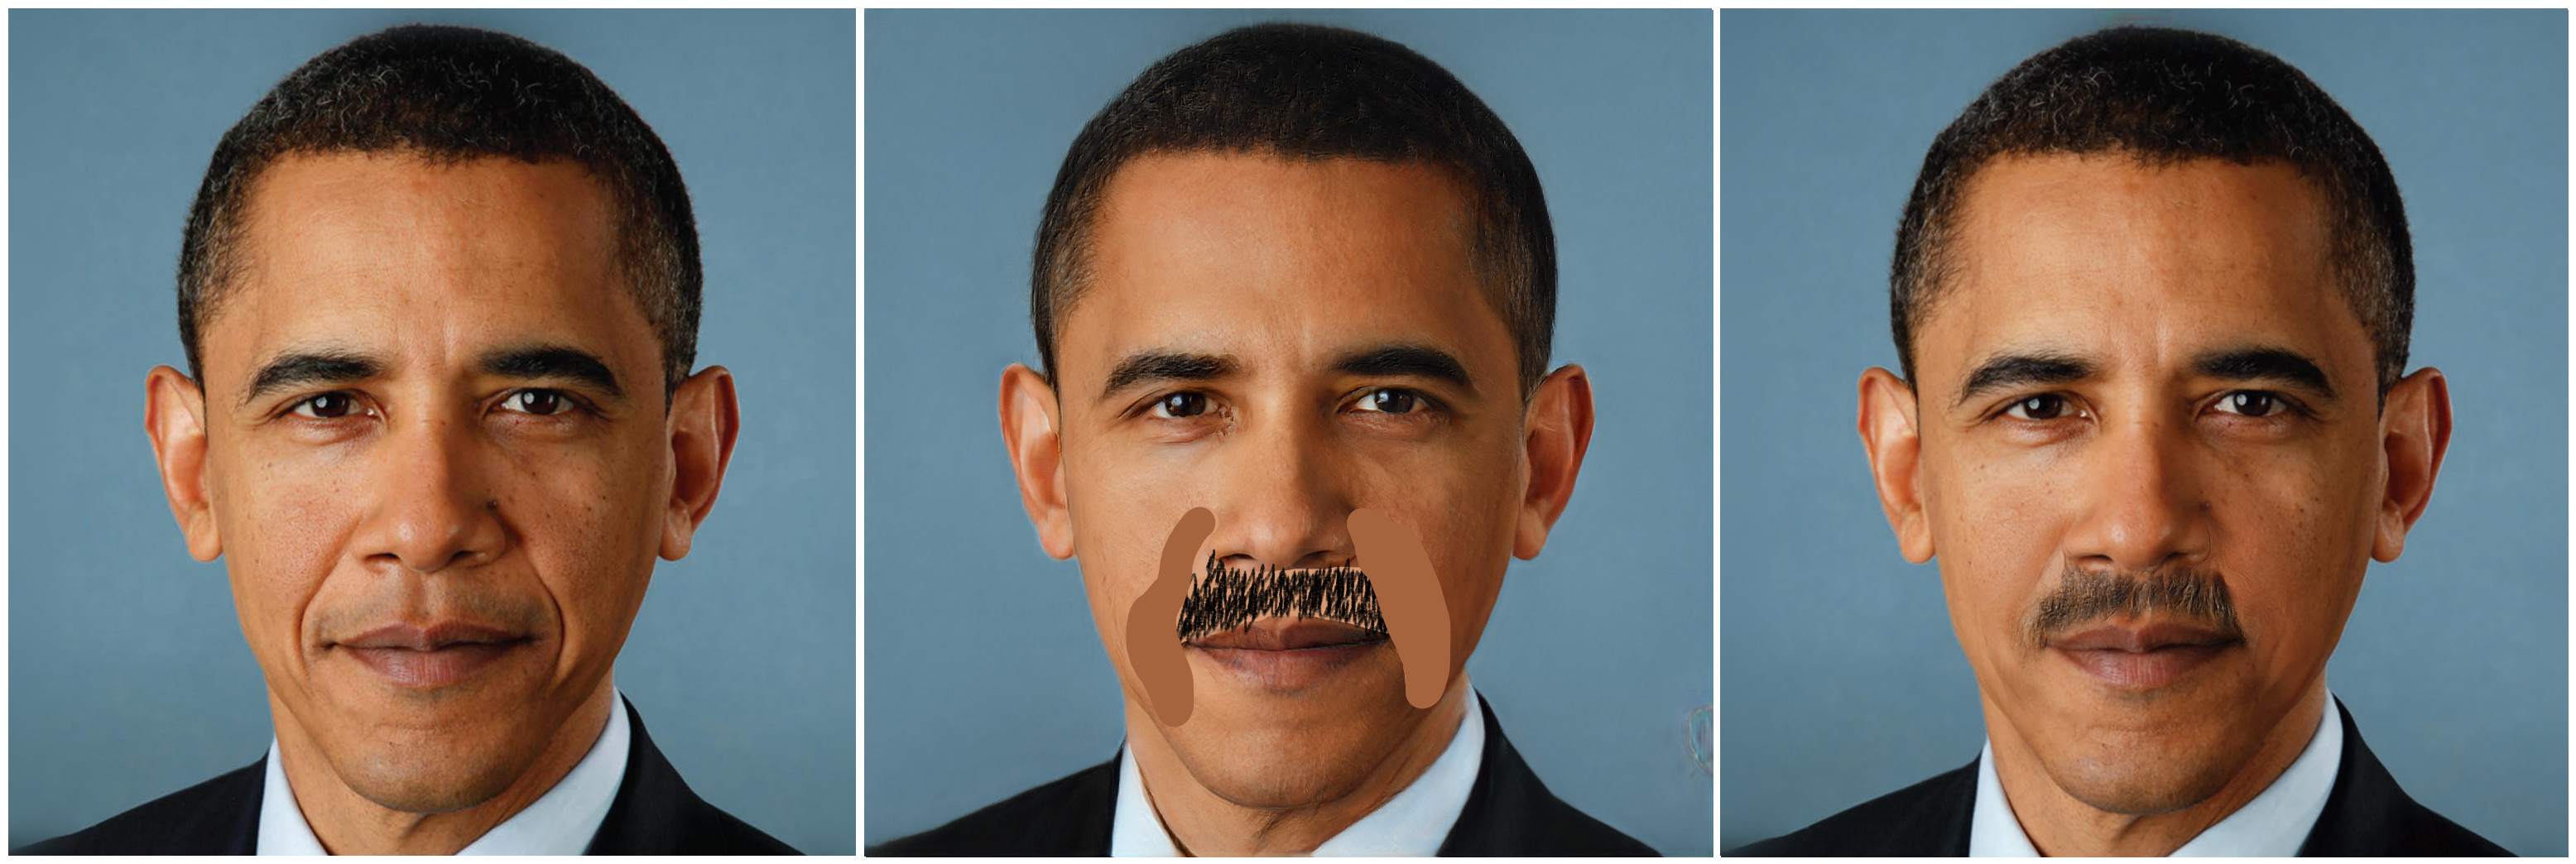
\includegraphics[width= 0.95\linewidth]{images/local_obama.jpg}
 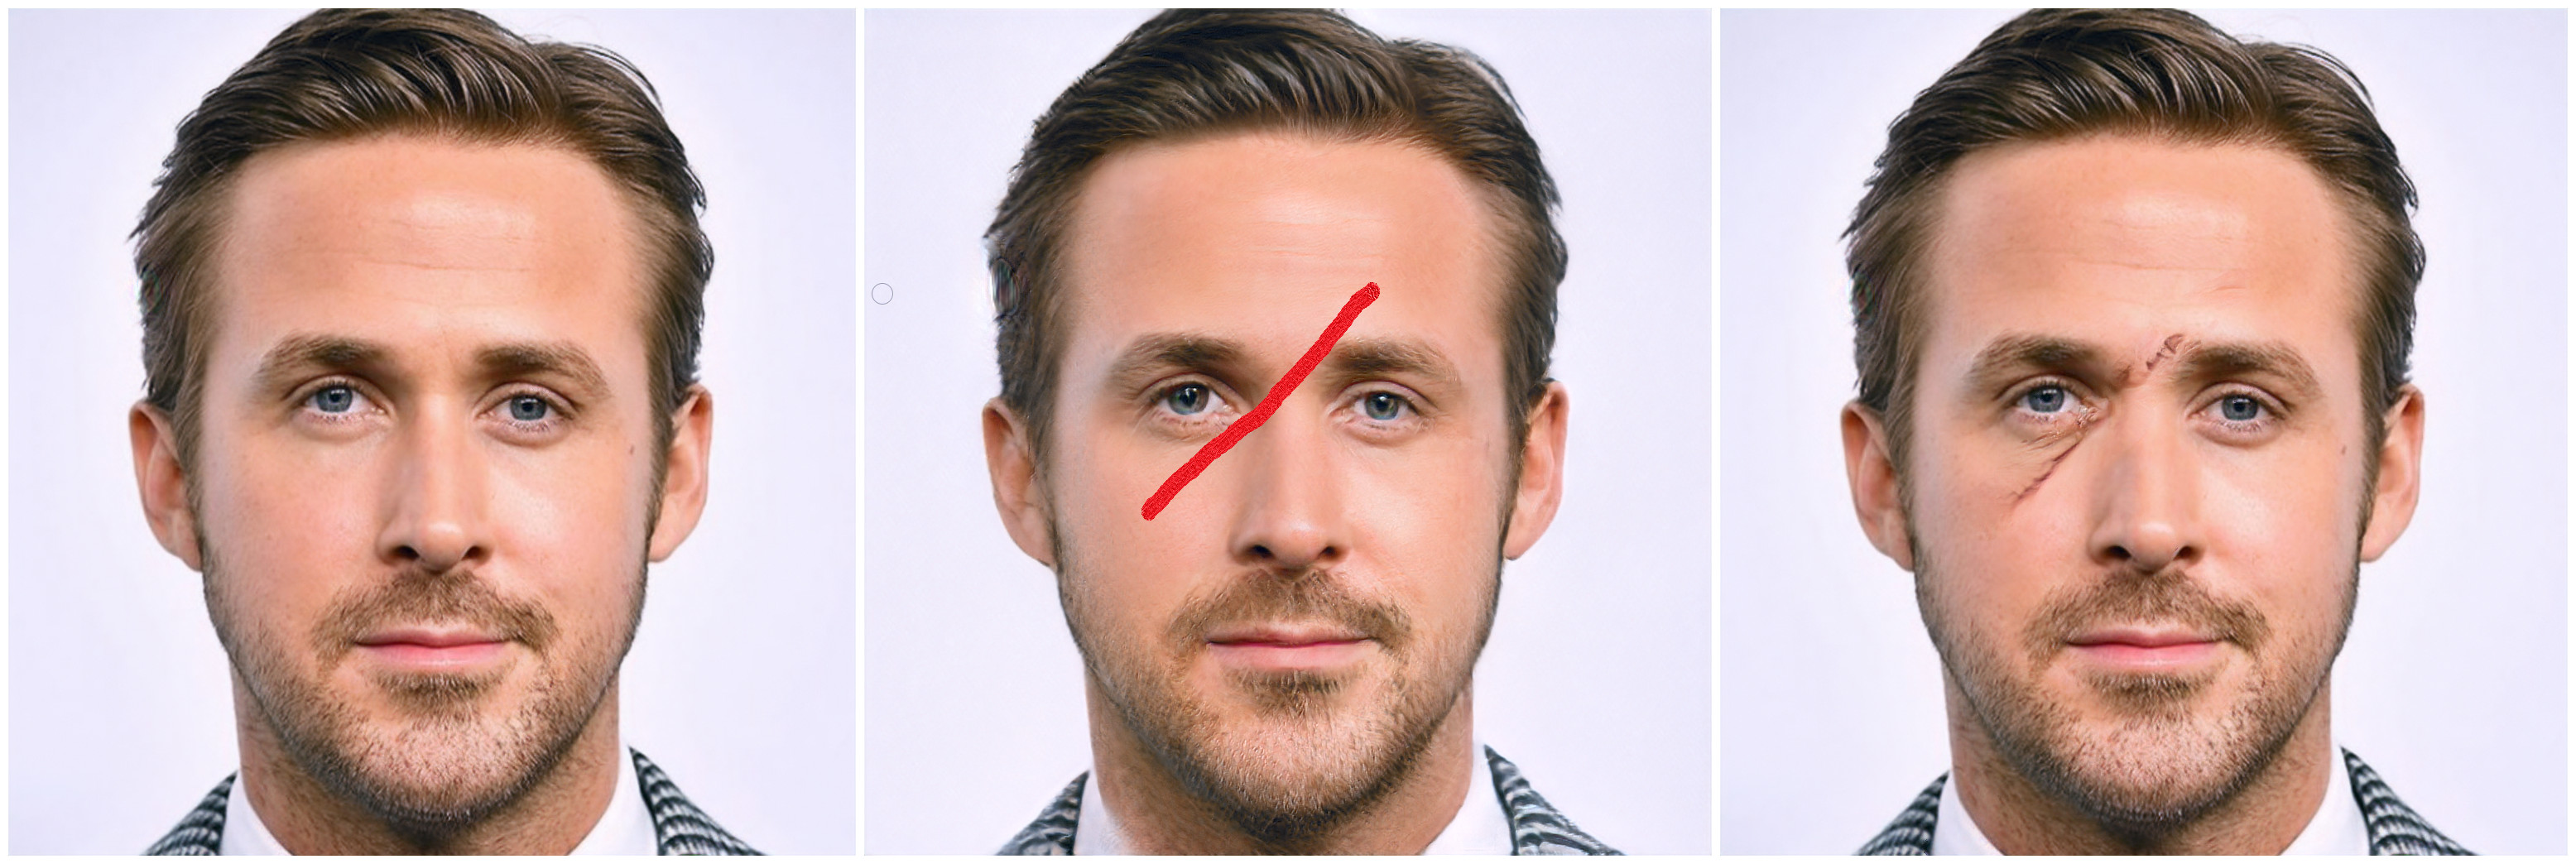
\includegraphics[width=0.95\linewidth]{images/local_ryan.jpg}
\caption{\textbf{兴趣区域编辑图解~\cite{abdal2020image2stylegan2}.} 从左到右: 基础模型; 涂鸦过的图像; 局部编辑的结果.}
\label{fig:local}
\end{figure}
}

\newcommand{\figrewrite}{
\begin{figure}[tbp]
\begin{center}
\includegraphics[width=0.95\linewidth]{images/ganrewriting}
\end{center}
\caption{\textbf{用于重写模型的复制-粘贴-上下文接口~\cite{zhu2016generative}.} 
%The first row is the user inputs and the last are corresponding model outputs. 
(a) 复制:用户使用笔刷选择一个区域包含一个有趣的对象或形状,定义目标. (b) 粘贴:用户定位和粘贴复制的对象到一个单一的目标图像. (c) 上下文:为了控制泛化,用户在几张图像中选择目标区域. (d) 编辑被应用到模型上,而不是应用到特定的图像上,这样新生成的图像就会在马头顶上有帽子. (e) 这种变化已经应用于不同类型的马和姿势.}
\label{fig:ganrewriting}
\end{figure}
}

\newcommand{\figood}{
\begin{figure}[tbp]
\begin{center}
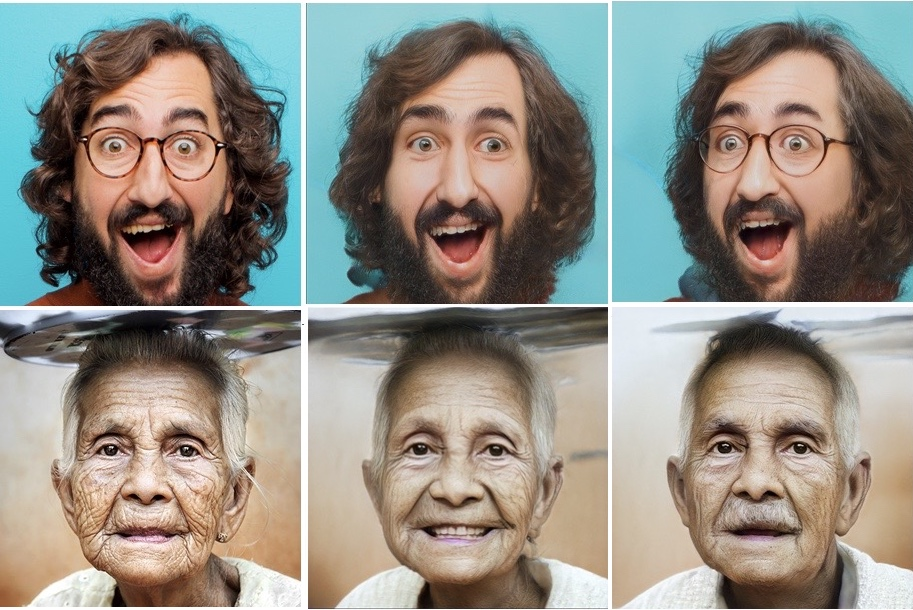
\includegraphics[width=0.95\linewidth]{images/ood}
\end{center}
\caption{\textbf{人脸图像处理的图解.} 这些是真实的图像编辑结果,来自StyleFlow~\cite{abdal2020styleflow}.}
\label{fig:ood}
\end{figure}
}

\newcommand{\figapp}{
\begin{figure}[tbp]
\begin{center}
\includegraphics[width=0.95\linewidth]{images/application_zhou}
\end{center}
\caption{\textbf{用GAN逆向进行图像处理的图解.}
GAN逆向不需要特定于任务的密集标记数据集,可以应用于许多任务,如图像重建、图像恢复和图像操作. 
% GAN inversion does not require task-specific dense-labeled datasets and can be applied to many tasks like image reconstruction (a), image restoration (b)(c)(d)(e) and image manipulation (f). 
The upper illustration (a) 来自 mGANPrior~\cite{gu2020image} 下面的(b) 来自DGP~\cite{pan2020exploiting}.}
\label{fig:application}
\end{figure}
}

\newcommand{\figcorrect}{
\begin{figure}[tbp]
\begin{center}
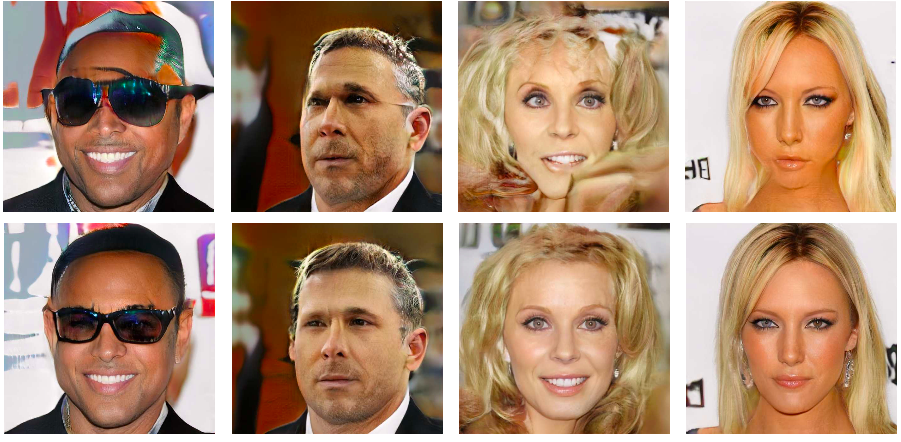
\includegraphics[width=0.98\linewidth]{images/correction}
\end{center}
\caption{\textbf{伪影校正结果.}  第一行显示的是PGGAN~\cite{karras2017progressive}生成的示例。第二行是通过将隐向量沿着正向质量方向移动而逐步修正的合成。此图来自~\cite{shen2020interpreting}.}
\label{fig:correction}
\end{figure}
}

\newcommand{\algotransfer}{
\begin{algorithm}[t]
\SetAlgoLined
\KwIn{images $x, y \in \mathbb{R}^{n \times m \times 3}$; masks $M_b$}
\KwOut{the embedded code $(\mathbf{w_o},\mathbf{n_o})$} 
$(\mathbf{w^*},\mathbf{n_i}) \leftarrow$ initialize()\;
{$\mathbf{w_o} = W_{l}(M_b,M_b,1 ,\mathbf{w^*},\mathbf{n_i},x)$\
$+ M_{st}(1-M_b,\mathbf{w^*} ,\mathbf{n_i}, y)$\;
$\mathbf{n_o} = {Mk}_{n}(M_b,\mathbf{w_o},\mathbf{n_i},x,G(\mathbf{w_o}))$\;
}
\caption{局部风格转移~\cite{abdal2020image2stylegan2}}
\label{alg:local_style_tranfer}
\end{algorithm}
}

\newcommand{\figtransfer}{
\begin{figure}[tp]
\centering
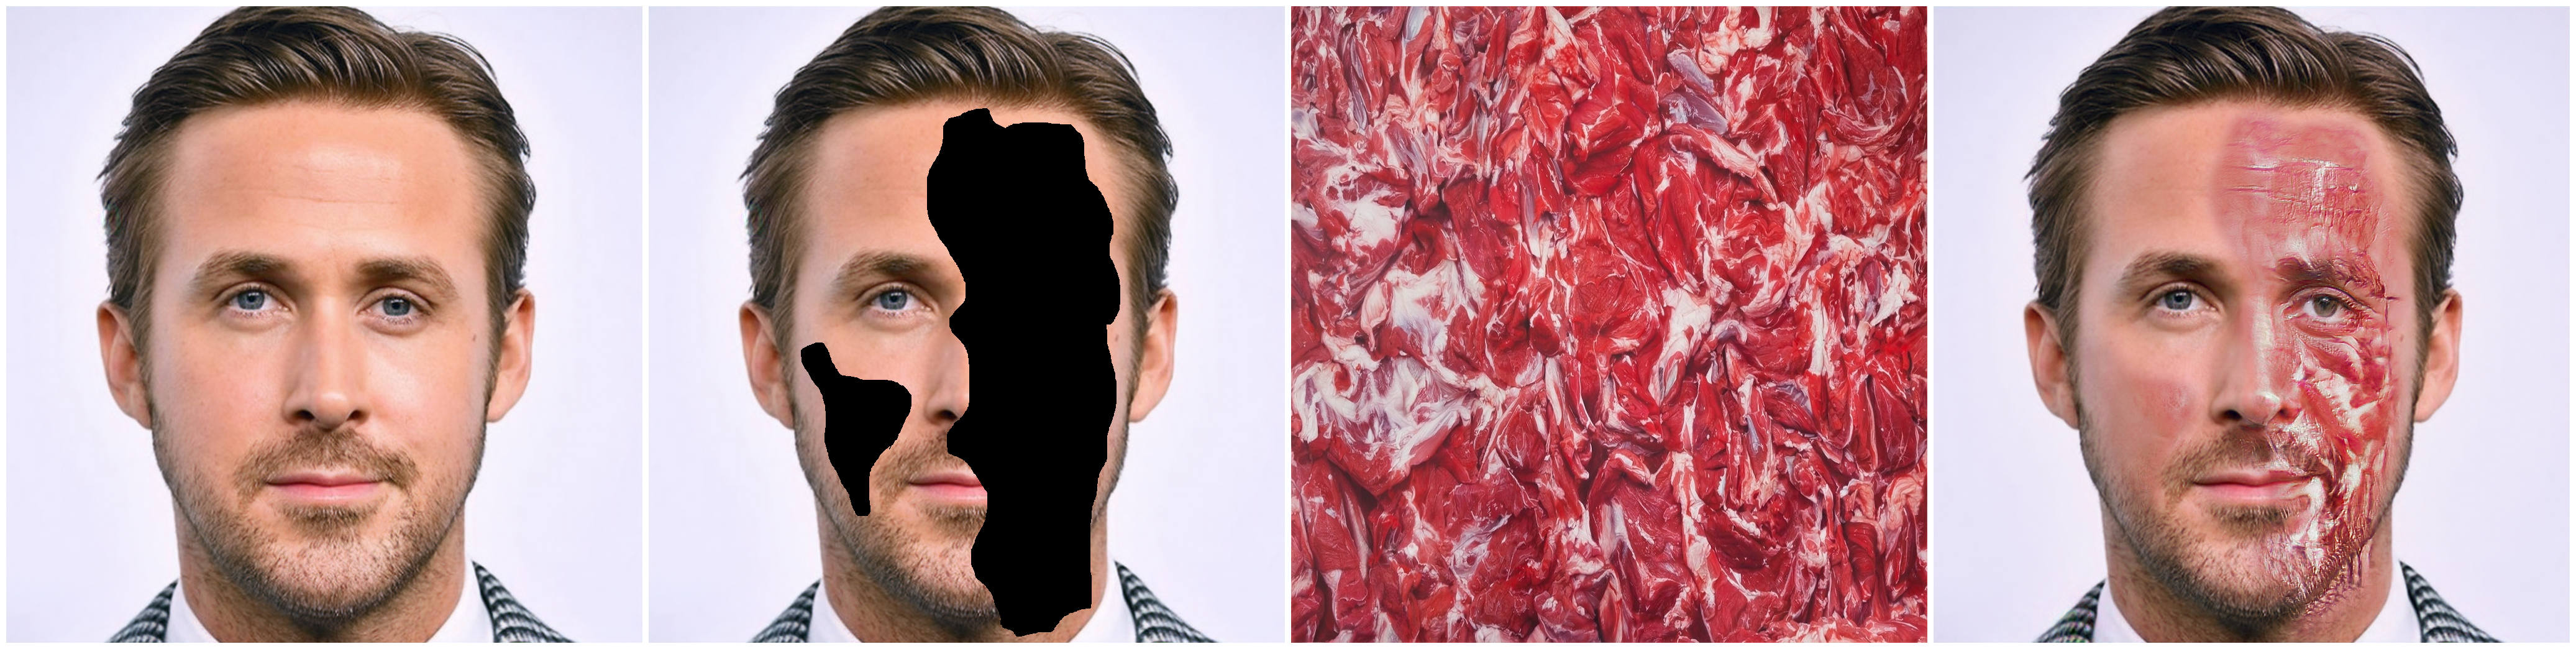
\includegraphics[width=0.95\linewidth]{images/style_ryan.jpg}
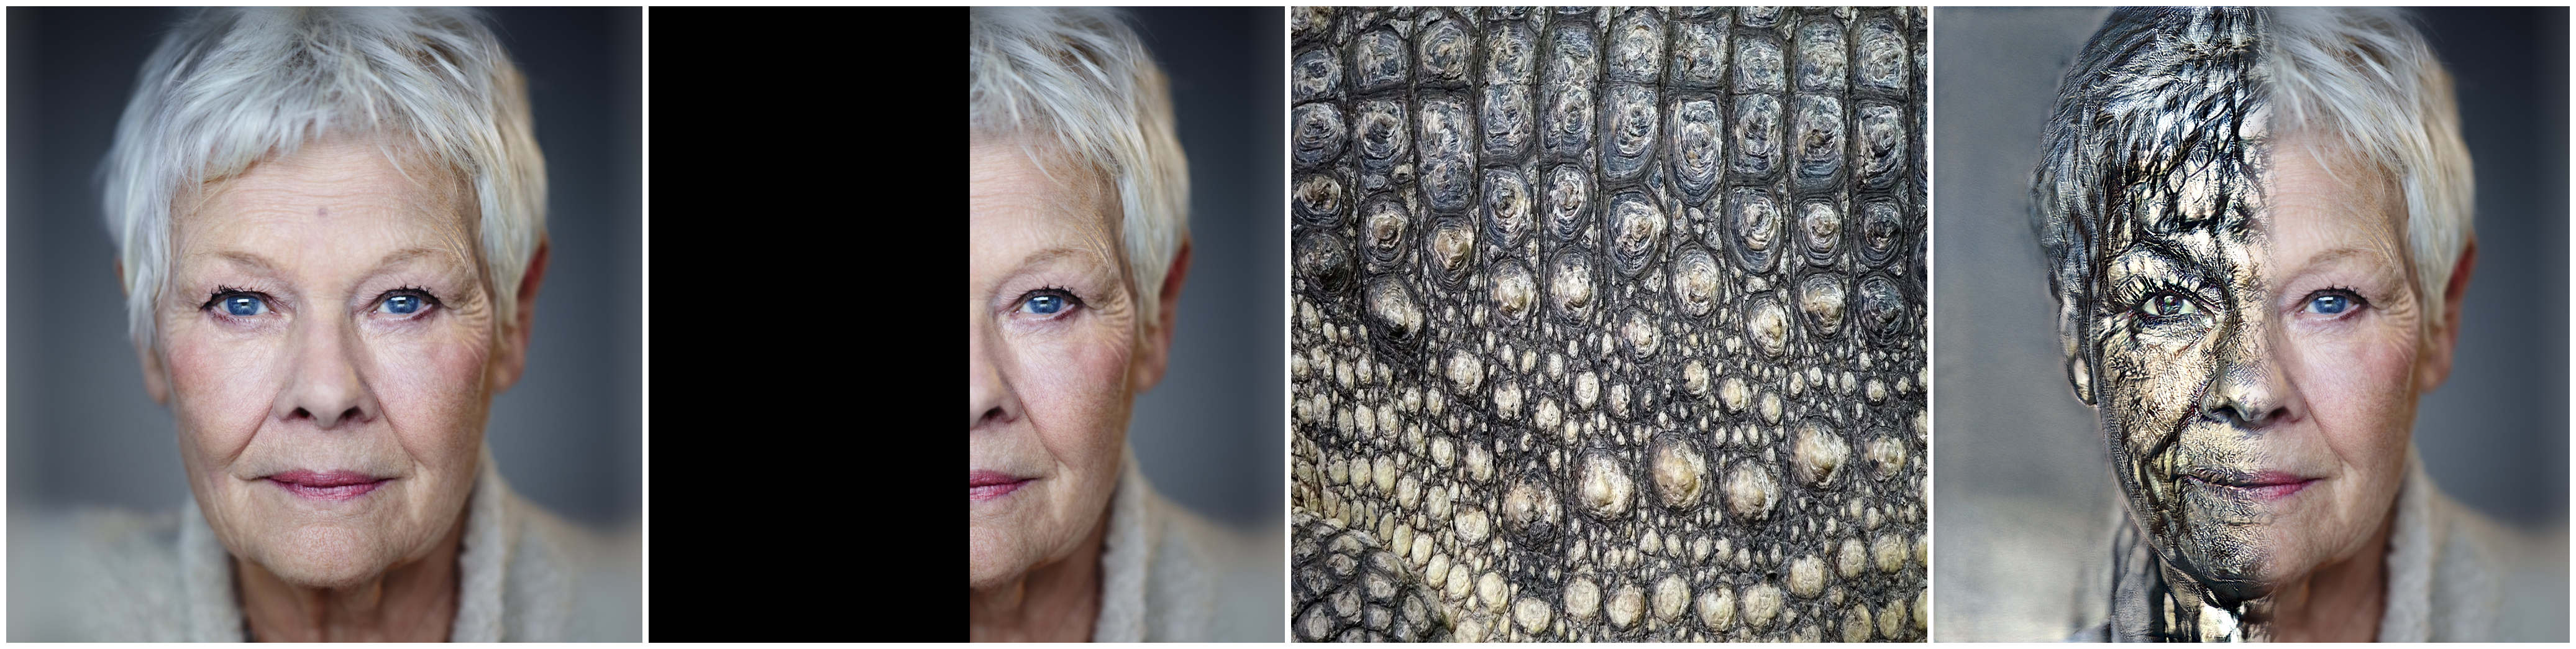
\includegraphics[width=0.95\linewidth]{images/style_judi.jpg}
\caption{\textbf{局部风格迁移图解~\cite{abdal2020image2stylegan2}.} 从左到右: 基础图像, 遮盖的区域, 风格图像, 局部风格迁移的结果.}
\label{fig:local_style_tranfer}
\end{figure}
}

\newcommand{\figinteractive}{
\begin{figure}[tbp]
\begin{center}
\includegraphics[width=0.95\linewidth]{images/interactive}
\end{center}
\caption{\textbf{使用GAN逆向进行交互式图像生成的图解.} (a) 插图结果来自 ~\cite{zhu2016generative}. 用户可以使用笔刷工具从零开始生成图像,并不断添加更多的涂鸦或草图以改进。最后一行显示了与生成的图像最相似的真实图像。虚线表示素描工具,彩色涂鸦表示颜色笔刷.
(b) 来自 GANPaint~\cite{bau2019ganpaint}. 笔刷可以绘制有语义意义的单元,如移走椅子或增加屋顶.
}
\label{fig:interactive}
\end{figure}
}

\newcommand{\figdiffusion}{
\begin{figure}[tbp]
\begin{center}
\includegraphics[width=0.95\linewidth]{images/diffusion.pdf}
\end{center}
\caption{\textbf{使用域内GAN逆向方法的语义扩散结果~\cite{zhu2020indomain}}. 第一列中的目标图像自然地扩散到第一行的上下文图像中,并保留标识.}
\label{fig:diffusion}
\end{figure}
}

\newcommand{\tabfeature}{
\begin{table*}[htbp]
\caption{逆向方法的特点. `Type' 包括基于学习的 (L.), 基于优化的(O.), 混合的(H.), 以及 封闭式的 (C.) GAN 逆向. I.-D., S.-A., L.-W., N.-I., R.-I. 和 O.-D. 分别表示发现可解释的方向(包括有监督的 (S.) 或无监督的(U.) 方式)、语义感知、逐层、非干涉的、感兴趣区域和分布外的特点. GAN模型和数据集表示哪个预训练的模型是在哪个数据集上,用哪个方法进行逆向的,这些可以在章节~\ref{sec:model_data}中找到.}
\label{tab:taxonomy}
\begin{center}
\scalebox{0.92}{
\begin{tabular}{c|c|c|c|c|c|c|c|c|c|c}
\toprule
Method  & Publication & Type &I.-D. &S.-A. &L.-W. &N.-I. &R.-I. &O.-D. &GAN Model & Dataset \\\hline
Zhu~\etal~\cite{zhu2016generative} &2016, NeurIPS &H. &\nxmark &\nxmark &\nxmark &\nxmark &\nxmark &\nxmark &\cite{radford2016dcgan} &\cite{yu2014local,zhou2014places,yu2015lsun}\\
Creswell~\etal~\cite{creswell2018inverting} &2018, TNNLS &O. &\nxmark &\nxmark &\nxmark &\nxmark &\nxmark &\nxmark &\cite{radford2016dcgan,gulrajani2017improved} &\cite{yu2014local,liu2015faceattributes}\\
GAN Dissection~\cite{bau2019gandissect} &2019, ICLR &O. &\nxmark &\ncmark &\ncmark &\nxmark &\ncmark &\nxmark &\cite{karras2017progressive} &\cite{yu2015lsun}\\
GAN Paint~\cite{bau2019ganpaint} & 2019, TOG &H. &\nxmark &\ncmark &\ncmark &\nxmark &\ncmark &\nxmark & \cite{karras2017progressive} & \cite{yu2015lsun}\\
Raj~\etal~\cite{raj2019gan} &2019, ICCV &O. &\nxmark &\nxmark &\nxmark &\nxmark &\nxmark &\nxmark &\cite{radford2016dcgan,zhang2019self} &\cite{yu2015lsun,lecun1998mnist,liu2015faceattributes}\\
GANSeeing~\cite{bau2019seeing} &2019, ICCV &H. &\nxmark &\ncmark &\ncmark &\nxmark & \nxmark &\nxmark &\cite{gulrajani2017improved,karras2017progressive,karras2019style}  &\cite{yu2015lsun}\\
Image2StyleGAN~\cite{abdal2019image2stylegan} &2019, ICCV &O. &\nxmark &\ncmark &\nxmark &\nxmark &\nxmark &\nxmark &\cite{karras2019style} &\cite{karras2019style} \\
Image2StyleGAN++~\cite{abdal2020image2stylegan2} &2020, CVPR &O. &\nxmark &\ncmark &\nxmark &\nxmark &\ncmark&\nxmark &\cite{karras2017progressive,karras2019style} &\cite{karras2017progressive,karras2019style}\\
mGANPrior~\cite{gu2020image} &2020, CVPR &O. &\nxmark &\ncmark &\ncmark &\ncmark &\nxmark &\ncmark &\cite{karras2017progressive,karras2019style} &\cite{karras2017progressive,karras2019style,yu2015lsun}\\
%IIN~\cite{esser2020invertible} &2020, CVPR &  &  &  &  &  &  &\\
Editing in Style~\cite{collins2020uncovering} &2020, CVPR &O. &\nxmark &\ncmark &\nxmark &\nxmark &\ncmark &\nxmark &\cite{karras2017progressive,karras2019style,karras2020analyzing} &\cite{karras2019style,yu2015lsun}\\
StyleRig~\cite{tewari2020stylerig} &2020, CVPR &L. &\nxmark &\ncmark &\nxmark &\nxmark &\nxmark &\nxmark &\cite{karras2019style} &\cite{karras2019style}\\
InterFaceGAN~\cite{shen2020interpreting} &2020, CVPR &L., O. &S. &\ncmark &\ncmark &\ncmark &\nxmark &\ncmark  &\cite{karras2017progressive,karras2019style} &\cite{karras2019style}\\
YLG~\cite{daras2020your} &2020, CVPR &O. &\nxmark &\nxmark &\nxmark &\nxmark &\nxmark &\ncmark &\cite{zhang2019self} &\cite{russakovsky2015imagenet}\\
GANRewriting~\cite{bau2020rewriting} &2020, ECCV &O. &\nxmark &\ncmark &\nxmark &\nxmark &\ncmark &\nxmark &\cite{karras2017progressive,karras2020analyzing} &\cite{yu2015lsun}\\
DGP~\cite{pan2020exploiting} &2020, ECCV &O. &\nxmark &\nxmark &\ncmark &\nxmark &\nxmark &\nxmark &\cite{brock2018large} &\cite{zhou2014places,russakovsky2015imagenet}\\
Huh~\etal~\cite{huh2020transforming} &2020, ECCV &O. &\nxmark &\ncmark &\nxmark &\nxmark &\ncmark &\ncmark &\cite{brock2018large,karras2020analyzing} &\cite{russakovsky2015imagenet,yu2015lsun,karras2019style}\\
IDInvert~\cite{zhu2020indomain} &2020, ECCV &H. &\nxmark &\ncmark &\nxmark &\nxmark &\nxmark &\ncmark &\cite{karras2019style}  &\cite{karras2019style,yu2015lsun}\\
StyleGAN2 Distillation~\cite{viazovetskyi2020distillation} &2020, ECCV &O. &S. &\ncmark &\nxmark &\ncmark &\nxmark &\ncmark &\cite{karras2020analyzing} &\cite{karras2019style}\\
GANSteering~\cite{jahanian2020steerability} &2020, ICLR &O. &S. &\ncmark &\nxmark &\nxmark &\nxmark &\nxmark &\cite{brock2018large,karras2019style,radford2016dcgan} &\cite{russakovsky2015imagenet,yu2015lsun,karras2019style}\\
GANLatentDiscovery~\cite{voynov2020latent} &2020, ICML &O. &U. &\ncmark &\nxmark &\nxmark &\nxmark &\nxmark &\cite{brock2018large,karras2017progressive} &\cite{karras2017progressive,jin2017towards,lecun1998mnist}\\
PIE~\cite{tewari2020pie} &2020, TOG &O. &S. &\ncmark &\nxmark &\ncmark &\nxmark &\ncmark &\cite{karras2019style}  &\cite{karras2019style}\\
StyleFlow~\cite{abdal2020styleflow} &2020, arxiv &O. &S. &\ncmark &\nxmark &\ncmark &\nxmark &\ncmark &\cite{karras2019style,karras2020analyzing}  &\cite{karras2019style,yu2015lsun}\\
GANSpace~\cite{eric2020GANSpace} &2020, arxiv &O. &U. &\ncmark &\ncmark &\ncmark &\nxmark &\nxmark &\cite{brock2018large,karras2019style,karras2020analyzing} &\cite{karras2017progressive,yu2015lsun}\\
Nitzan~\etal~\cite{nitzan2020harness} &2020, arxiv &L. &\nxmark &\ncmark &\nxmark &\ncmark &\nxmark &\nxmark &\cite{karras2019style}  &\cite{karras2017progressive,karras2019style}\\
% Li~\etal~\cite{li2020latent} &2020, arxiv &O. &\nxmark &\ncmark &\nxmark &\ncmark &\nxmark &\nxmark &\cite{gulrajani2017improved}  &\cite{xiao2017fashion,yu2017jittor}\\
SeFa~\cite{shen2020closedform} &2020, arxiv &C. &U. &\ncmark &\ncmark &\ncmark &\ncmark &\ncmark &\cite{karras2017progressive,brock2018large,karras2019style,karras2020analyzing} &\cite{naik2014streetscore,karras2017progressive,karras2019style,yu2015lsun,russakovsky2015imagenet}\\
Aberdam~\etal~\cite{aberdam2020invert} &2020, arxiv &O. &\nxmark &\nxmark &\ncmark &\nxmark &\nxmark &\nxmark & a two-layer model & \cite{lecun1998mnist} \\
StyleGAN-Encoder~\cite{guan2020faster} &2020, arxiv &L. &\nxmark &\ncmark &\nxmark &\ncmark &\nxmark &\nxmark &\cite{karras2019style} &\cite{karras2017progressive,karras2019style,chen2014cross}\\
GH-Feat~\cite{xu2020ghfeat} &2020, arxiv &L. &\nxmark &\ncmark &\ncmark &\nxmark &\nxmark &\nxmark &\cite{karras2019style} &\cite{lecun1998mnist,yu2015lsun,karras2019style}\\
pSp~\cite{richardson2020encoding} &2020, arxiv &L. &\nxmark &\ncmark &\ncmark &\ncmark &\ncmark &\ncmark &\cite{karras2020analyzing} &\cite{karras2017progressive}\\
Style Intervention~\cite{liu2020style} &2020, arxiv &O. &S. &\ncmark &\nxmark &\ncmark &\ncmark &\ncmark &\cite{karras2020analyzing} &\cite{liu2020style}\\
StyleSpace~\cite{wu2020stylespace} &2020, arxiv &O.&S. &\ncmark &\nxmark &\ncmark &\ncmark &\ncmark &\cite{karras2020analyzing} &\cite{karras2019style,yu2015lsun}\\
Lu~\etal~\cite{lu2020discovery} &2020, arxiv &L. &U. &\ncmark &\nxmark &\ncmark &\nxmark &\nxmark &\cite{karras2020analyzing,karras2017progressive,miyato2018spectral} &\cite{karras2019style,russakovsky2015imagenet}\\
Cherepkov~\etal~\cite{cherepkov2020navigating} &2020, arxiv &O. &U. &\ncmark &\nxmark &\ncmark &\nxmark &\ncmark &\cite{karras2020analyzing} &\cite{karras2019style,yu2015lsun}\\
Nurit~\etal~\cite{nurit2020steerability} &2020, arxiv &C. &U. &\ncmark &\nxmark &\ncmark &\nxmark &\nxmark &\cite{brock2018large} &\cite{russakovsky2015imagenet} \\

\bottomrule
\end{tabular}
}
\end{center}
\end{table*}
% \footnotetext[1]{They use a self-defined two-layer GAN model.}
}